\chapter{Evaluating a time notification on interruptions}

\begin{mynote}
\subsubsection{Chapter outline}
This chapter describes two studies that, given varying IACs, evaluate whether giving people feedback on the duration of their switches can influence people's switching strategies and data entry performance. A browser notification was developed which showed people how long they switch away for on average. Study 6 evaluates the notification with an experimental task, to see if time information influences the strategies people adopt, and can make people adopt more accurate and faster. Study 7 evaluates the notification in the office setting with workers doing data entry work, to ascertain how appropriate the proposed recommendations are for a naturalistic task for which they would be used.

Together these studies intend to show that time information makes people switch less between entering and looking up information, which makes them faster to complete the data entry task overall and can reduce errors.
\end{mynote}

\section{Chapter introduction}
Chapter 3 presented two qualitative studies that investigated how office workers perform data entry work in office settings. It revealed that self-interruptions to collect information is a major aspect of their work. Even though data workers tried to collect information carefully before starting a task, they often did not realise they needed certain information until starting the task. Whereas they deferred retrieving physical sources, for digital sources they self-interrupted their task immediately to retrieve additional information. The hypothesis was made that differences in expected time costs influenced people's decisions on when to switch and interrupt themselves.

Chapter 4 presented findings from three controlled experiments that supported the hypothesis: when time costs to access digital sources are consistent, and people learn and anticipate the time it will take them to retrieve information, they will look up and enter items that take the least time first, and postpone getting information that takes time to look up. An issue is that, outside of a controlled setting, people often do not know how long an interruption to look up digital information may take, and whether they should switch immediately or later. As was observed in Study 2, digital interruptions often took far longer than intended because people had to search through large and multiple documents, and could get distracted by irrelevant information. Because they did not know the time they spent on task interruptions, it was difficult to manage these self-interruptions. 

The studies presented in this chapter aim to investigate whether giving people feedback on the time spent on task interruptions has any effect on people's self-interruptions. In particular, the purpose is to see whether time information reduces the number and duration of interruptions, and as a result can improve data entry performance. Study 6 used an experimental data entry task to measure if a notification showing the average duration on people's window switches had an effect on number and duration of their switches, and data entry speed and accuracy. Study 7 evaluated the feedback with data workers doing expenses work, to evaluate if the notification would be suitable for an applied task.


\section{Study 6: Looking up information in email during an online experiment}

\subsection{Introduction}
%BRIDGE WITH LAST CHAPTER
\begin{comment}
The findings of the previous studies will have given insight into the influence of IAC on people's strategies of managing looking up information and how different strategies may be more efficient and accurate than others. For example, one finding can be that people who look up information from high IAC sources as they need it are slower and make more data entry errors than people who first collect all information and then enter it all in one sequence. 
It will have highlighted some functionalities that a data entry expenses system needs to offer users. These findings are translated into a set of requirements. These are used to test the existing system against, and used to develop possible future design recommendations suited to the task of entering expenses. 

The design recommendations will take into account both findings from Study 3 and 4 on what influences people's strategies and what is desirable, as well as the setting studied in Study 1 and 2 and what is feasible. For example, desired changes in the actual interface may be too expensive to be realistic, and it may be more feasible to change the way information sources are designed, or how these are laid out in the user's environment. Screenshots of the current interface system will be used (initial ones were obtained in Study 1, additional ones will be obtained in Study 2). 

Study 5 aims to test different designs in a controlled experiment, to investigate if changing design features influences people's switching strategies and their speed and accuracy in data entry. It will use the same task paradigm as Study 4 and compare different designs, to see if these changes have an influence on the strategies people adopt in looking up information for a data entry task, and whether these changes can make people adopt strategies that improve accuracy. 

Observations in Study 2 showed that data workers prepare some information they need for a data entry task beforehand. Other data items are retrieved as the task goes along. As soon as they realise they need information, they interrupt themselves and this can happen frequently during a single task. Finding information can take longer than expected, and people can get distracted along the way. In general, finding information is disruptive: people may forgotten where they were in a task, enter information in the wrong fields, or they might be automatically logged out of a system because of inactivity. Study 4 and 5 showed that in a controlled setting where people know the time it will take them to retrieve information, they adapt and schedule their tasks accordingly. They will look up and enter items that take the least time first, and postpone getting information that is difficult to lookup. An issue is that people often do not know how long it will take them and therefore cannot schedule or adapt to it. Can people be nudged into making more mindful interruptions, if they are given feedback on how long it takes them to find information?


A number of laboratory studies have looked at how people decide when to address interruptions. These studies showed that people defer interruptions until lower workload moments \citep{Salvucci2010}, or switch to another task when there is a delay in the primary task \citep{Gould2016, Katidioti2013}. However, these studies primarily focused on characteristics of the primary task, and it is unclear from these studies if the time taken to address an interruption has any effect. Study 4 and 5 showed that if the time to access data items for a data entry task is consistent throughout a controlled experiment, participants learn to look up and enter easy-to-access items first, before looking up other items. Might people therefore manage their interruptions differently, if they are given feedback on how long it takes them to find information?

\citet{Gould2016a} looked at people's switches to other, unrelated activities during an online routine data entry task. They found that a cue that asked participants to remain focused on the task after they switched reduced self-interruptions. The aim of the two studies in the current chapter was to see if a cue which indicates the duration of an interruption has any effect on people's switches to a related activity: look up information for a data entry task. Study 6 used an experimental data entry task to measure if a notification showing the average duration on people's switches had an effect on number and duration of their switches, and data entry speed and accuracy. Study 7 evaluated the feedback with data workers doing expenses work, to evaluate if the notification would be suitable for an applied task.

\end{comment}

%INTRODUCTION TO CURRENT
This study aimed to investigate whether an intervention showing people how long they switch on average has an effect on the duration and number of switches during a data entry task. An online experiment was conducted where participants had to complete a data entry task. Participants had to enter numeric codes into a form, which they had to retrieve from a message sent to their personal email. The information was presented as a message in participants' email inboxes, as email is an integral part of data entry work but known to be a source of distraction, and people often spend more time on it than originally intended \citep{Hanrahan2015, Mark2016}. It was therefore expected to have a distracting effect during the switches to look up information. Half of the participants received feedback on the average length of their switches through a browser notification. 
The research questions that this study aims to address are whether feedback on interruption length:

\begin{itemize}
\item
reduces the number of switches?
\item
 reduces the duration of switches?
\item
makes people faster in data entry?
\item
makes people more accurate in data entry?
\end{itemize}

\subsection{Method}
\subsubsection{Participants}
Fourty-seven participants (30 women) took part in the online experiment. Ages ranged from 20 to 63 (M = 29.3 years, SD = 9.1 years). The participants were recruited via university email lists, social media and online platforms to advertise academic studies, and participation was voluntary. Participants were alternately allocated to the control or experimental condition.

\subsubsection{Design}
The study used a between-participants design with one independent variable, a notification. In the control condition, participants did not receive a notification, but switches away from the data entry window were recorded. In the notification condition, participants were shown a notification every time they completed a trial. This notification showed how long on average they were away for when switching away from the window, before returning to the task. The purpose of this notification was to see if the number and duration of switches could be reduced by giving participants feedback on the time spent of on switches. Dependent variables were number and duration of switches away from the data entry interface, trial completion time, and data entry errors. Switching behaviour was recorded using JavaScript's blur and focus events. These were triggered whenever a participant switched away from the data entry window, whether to their email inbox or to a different window or application. 

\subsubsection{Materials}
The task used was based on a common routine data entry task from Study 1 and 2 involving processing expenses. Participants were presented with an online sheet containing a set of ten 'expenses' (see Figure 1). They had to complete each row by entering the correct expense code for the expense. They retrieved this code by looking it up in a table of 25 expense categories which each had a corresponding 5-digit expense code, shown in Figure 2. Participants had to determine which category an expense belonged to, look up the code of this category and enter it in the row of the expense. We used expense categories and codes that are currently used by a public university to process expenses.

In the example of Figure 1, the expense in the top row belongs to the category 'Postage' and the participant would have to copy the code 22104 from the expense table into the empty cell of the top row. A code did not occur more than once in a trial. The codes within a trial could be entered in any order. 
Once the codes of the ten expenses had been entered, participants clicked the Next button to go to the next trial and the sheet was filled with ten new expenses. Participants were not alerted to any mistakes and once they had pressed 'Next', they could not return to the previous trial to correct any errors. Participants had to complete one practice trial, and five experimental trials. The purpose of the practice trial was for the participant to get familiar with the task, and the recorded data from this trial was excluded from the analysis.

The experiment was conducted in a web browser. In addition to the main task, we implemented a browser notification that appeared when participants in the notification condition switched away from the data entry window (see Figure 3). Every time participants switched, a notification appeared at the right-hand corner of their screen that told participants how long on average they go away for when they switch. The notification stayed visible for several seconds as set by default by the browser, or participants could dismiss the notification themselves by clicking on it.

\begin{figure}
\centering
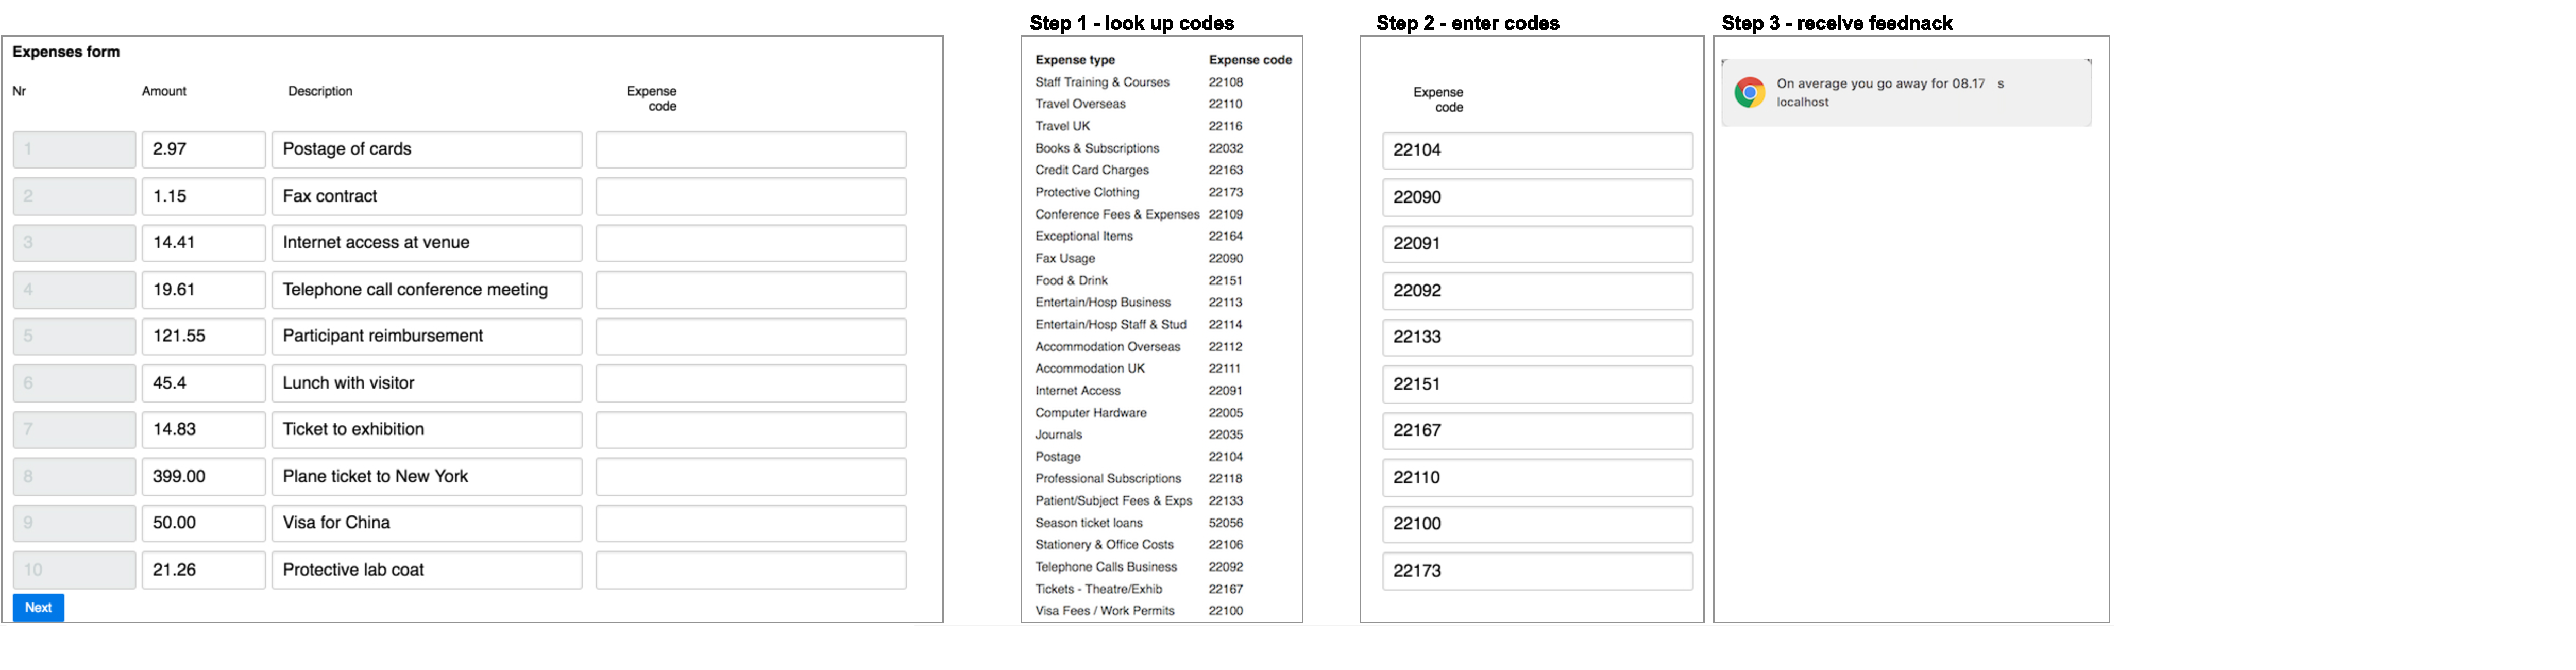
\includegraphics[width=\textwidth]{images/ch56/ch56-taskinterface.pdf}
\caption{The data entry task as shown in the browser. Participants had to look up codes from their email (Step 1) and enter this into a sheet (Step 2). After every trial, the notification condition received time information (Step 3)}
%\vspace{-3pt}
\label{fig:ch56-Figure1}
\end{figure}

\subsubsection{Procedure}
The study was advertised online with a brief description and a website link to sign up. Participants signed up for the experiment by entering their email address, and were sent an email with the table of expense categories and expense codes. The email also included instructions with a new link where the study was available. Participants were asked to complete the task on a desktop or laptop computer and open the experiment in Google Chrome, Firefox or Safari. Participants were not informed beforehand which condition they had been allocated to, and were told the purpose of the study was to understand how people perform data entry tasks. Participants in the notification condition were informed that they would receive notifications during the experiment. 
Participants first read an online consent form on the website, and were not able to continue to the experiment until they had agreed to the consent form. Participants in the notification condition received an additional dialog box to enable notifications in their browser, and had to click 'OK' to continue. Participants were instructed to have both their email and data entry window open on the same device, and to keep both windows maximised at all time, to ensure they had to switch back and forth between the two windows. Participants who made no recorded switches would be excluded from the dataset. 
After completing all experimental trials, participants were shown a page of debriefing information, explaining the purpose of the study. An email address was included as a point of contact if participants had any further questions. Participants took between 10 and 20 minutes to complete the experiment.

\subsubsection{Pilot study}

\subsection{Results}
Table \ref{tbl:ch56-Table1} summarises the results of the conditions in terms of the four dependent variables. The number of switches, length of switches and the error rate were not normally distributed, so non-parametric Mann-Whitney tests were used to analyse effects of a notification on these dependent variables. A Shapiro-Wilk test suggested that the trial completion times were normally distributed, \textit{W} = 0.97, \textit{p} = 0.22, so an independent t-test was used to analyse the effect on trial times. 

\subsubsection{Number and duration of switches}
Figure \ref{fig:ch56-Figure2} shows the variability of duration of switches for the two conditions. Results show that switches were significantly shorter among participants who had a notification (\textit{M} = 4.76s, \textit{SD} = 1.65s) than among those without a notification (\textit{M}=7.13s, \textit{SD}=3.05s), \textit{U} = 406, \textit{p} < 0.01, \textit{r}=.44. Participants switched once for every code entered (i.e., ten times per trial), and there was no significant difference in number of switches between conditions, \textit{U} = 243, \textit{p} = 0.6.

The distribution of switching durations was positively skewed with a long tail: switches up to 11 seconds made up 90\% of switches, but the longest switch was greater than seven minutes. The distribution of the top 10 \% of longest switches is illustrated in Figure \ref{fig:ch56-histswitches}. 
Table \ref{fig:ch56-tblswitches} shows the count of extremely long switches per condition.

\begin{figure}
\centering
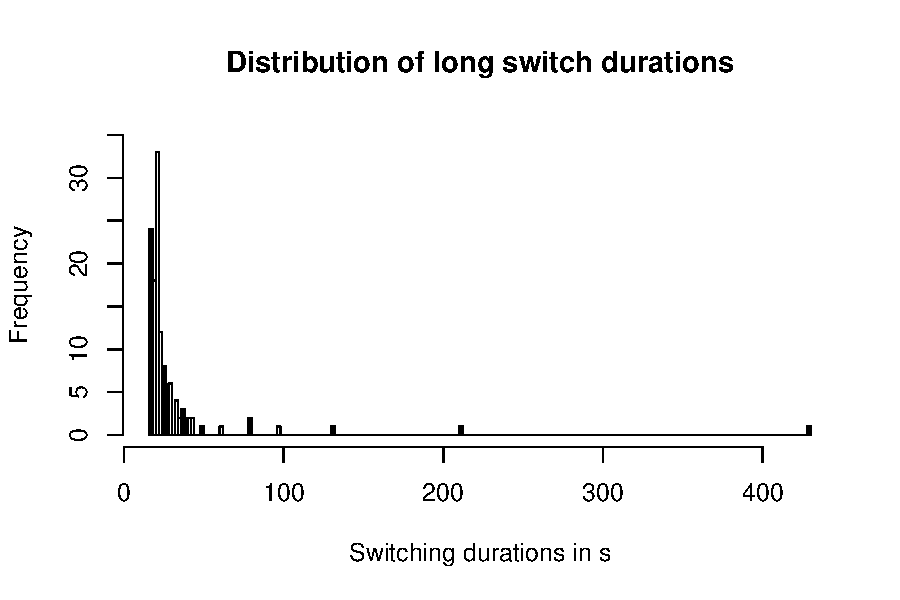
\includegraphics[width=\textwidth]{images/ch56/ch56-histswitches.pdf}
\caption{Distribution of the top 10\% longest window switches, that is switches that were longer than 11.82 seconds.}
%\vspace{-3pt}
\label{fig:ch56-histswitches}
\end{figure}

\begin{table}
\caption{Total number of switches at different percentiles for each condition.}
\centering
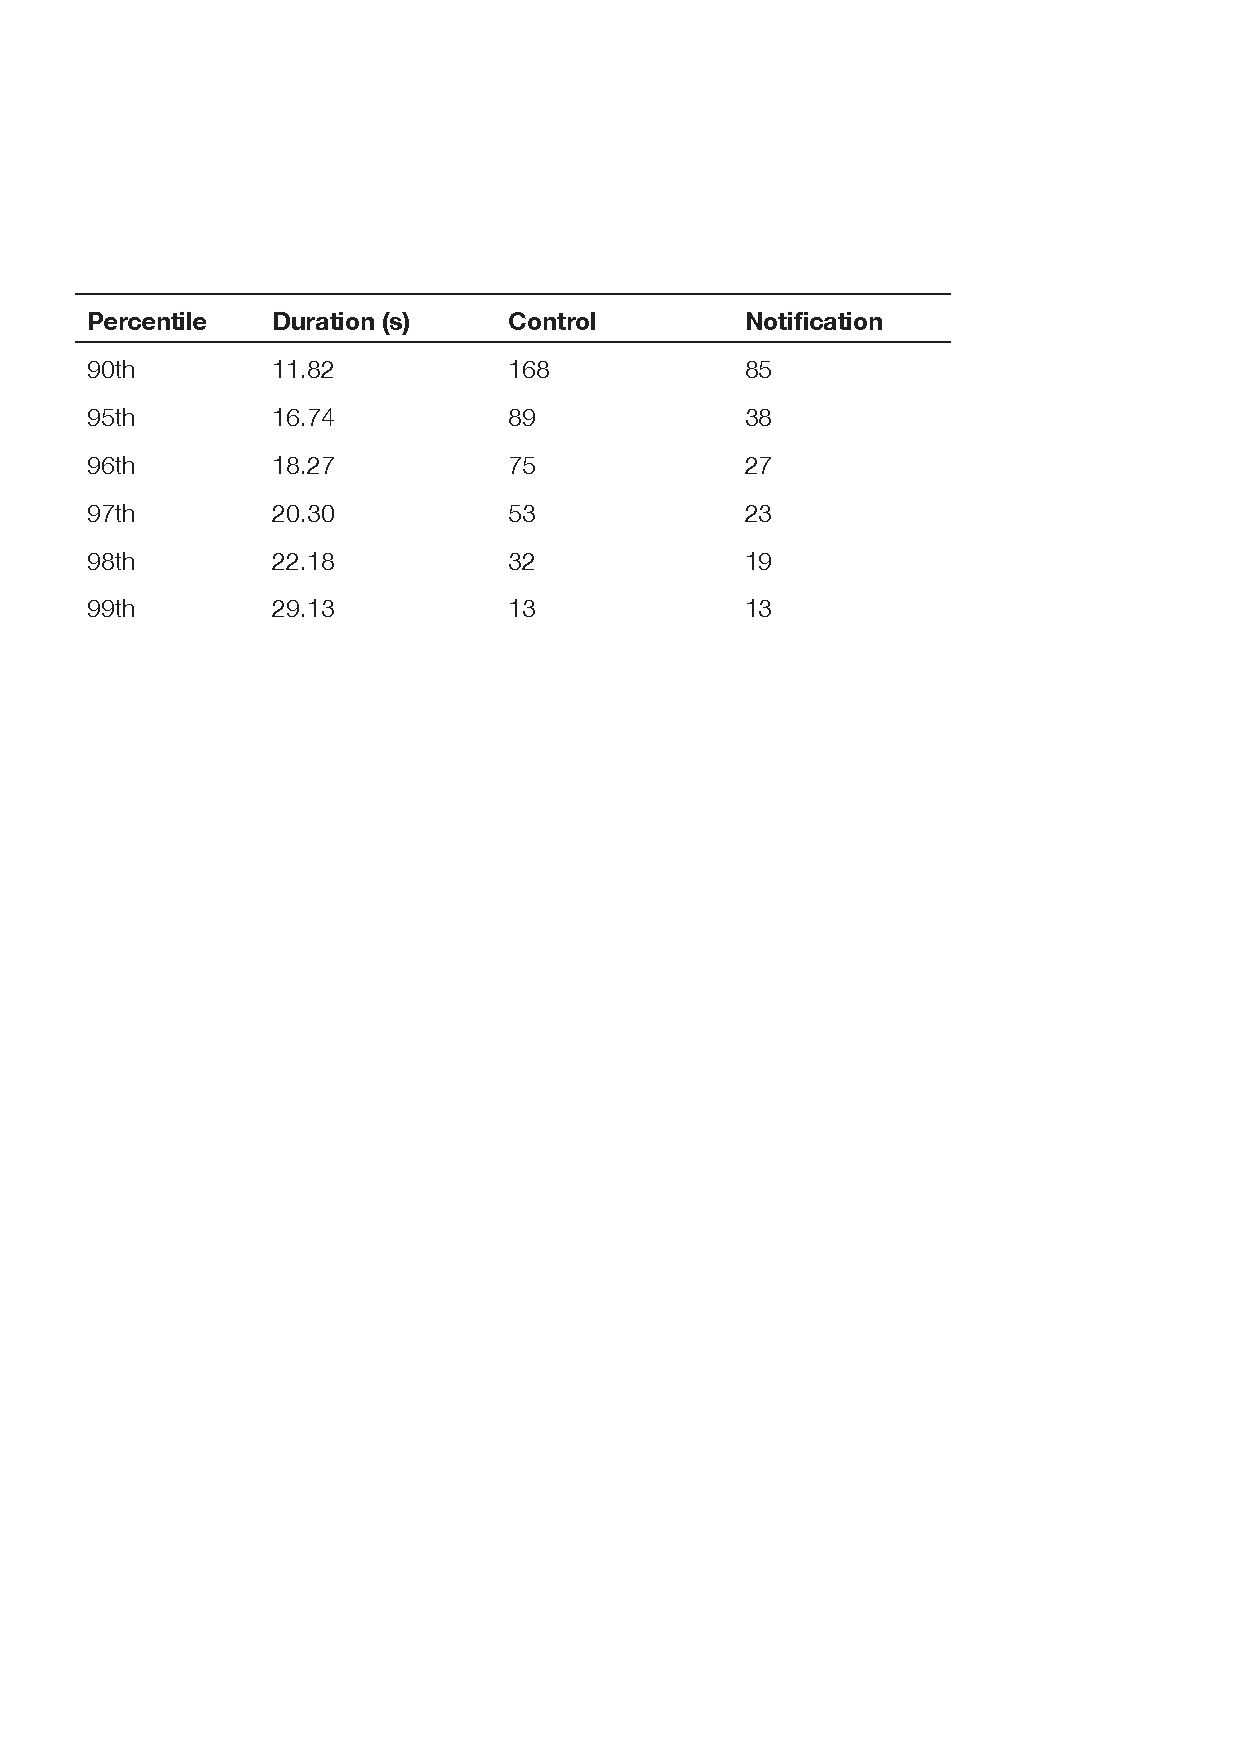
\includegraphics[width=0.7\textwidth]{images/ch56/ch56-longswitches.pdf}
\vspace{-3pt}
\label{tbl:ch56-tblswitches}
\end{table}


\subsubsection{Task performance}
Error rates were calculated by dividing the number of data entry errors divided by error opportunities. The error rates were significantly lower for participants with a notification (\textit{M }= 2\%, \textit{SD} = 2\%) compared to participants who had no notification (\textit{M} = 5\%, \textit{SD }= 5\%), \textit{U} = 403, \textit{p} < .01, \textit{r} = .44. Participants with a notification were also faster in completing trials (\textit{M} = 107.61s, \textit{SD} = 31.15s) compared to participants without a notification (\textit{M} = 126.27s, \textit{SD} = 32.61), \textit{t}(45) = 1.98, \textit{p} < .05, \textit{d} = .59.

\begin{table}
\caption{Means and standard deviations of dependent variables for each condition.}
\centering
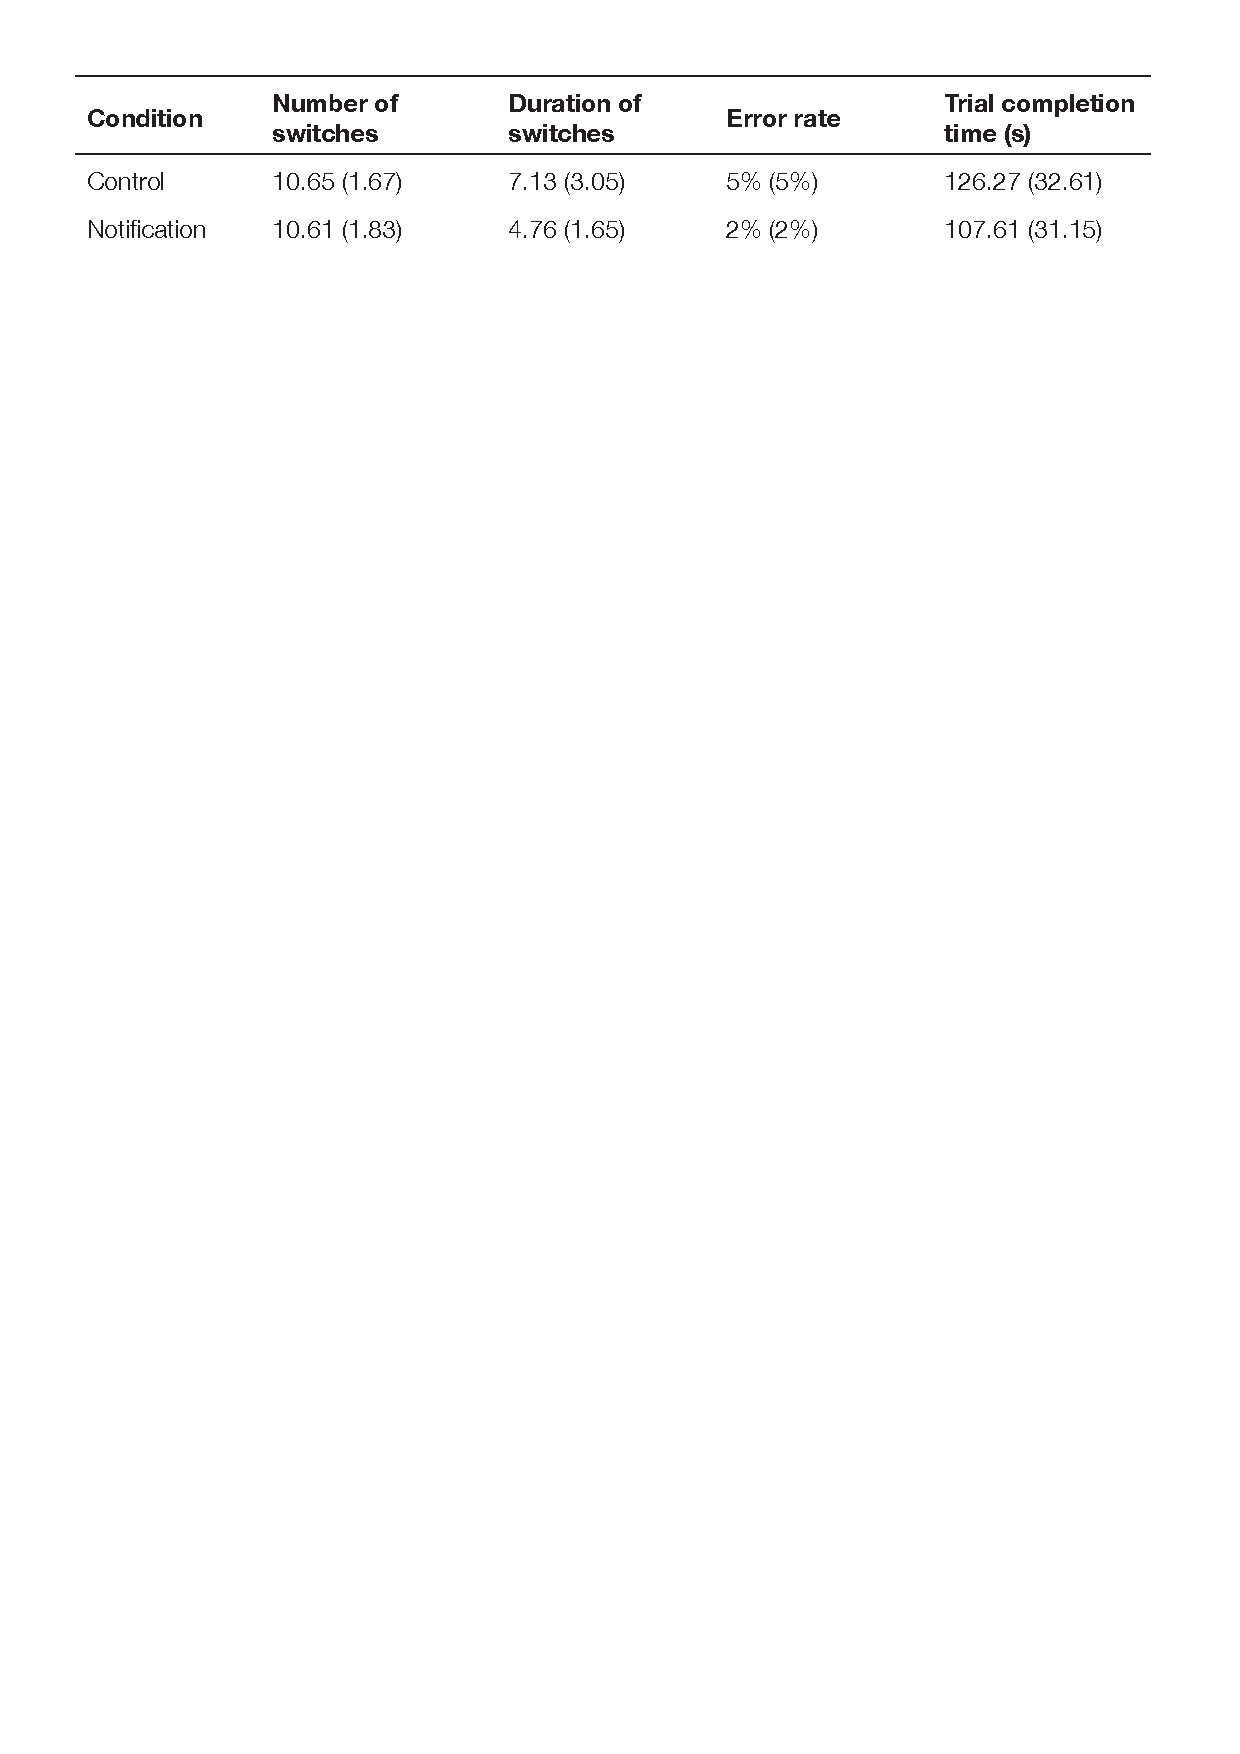
\includegraphics[width=0.9\textwidth]{images/ch56/ch56-descstats.pdf}
\vspace{-3pt}
\label{tbl:ch56-Table1}
\end{table}

\begin{figure}
\centering
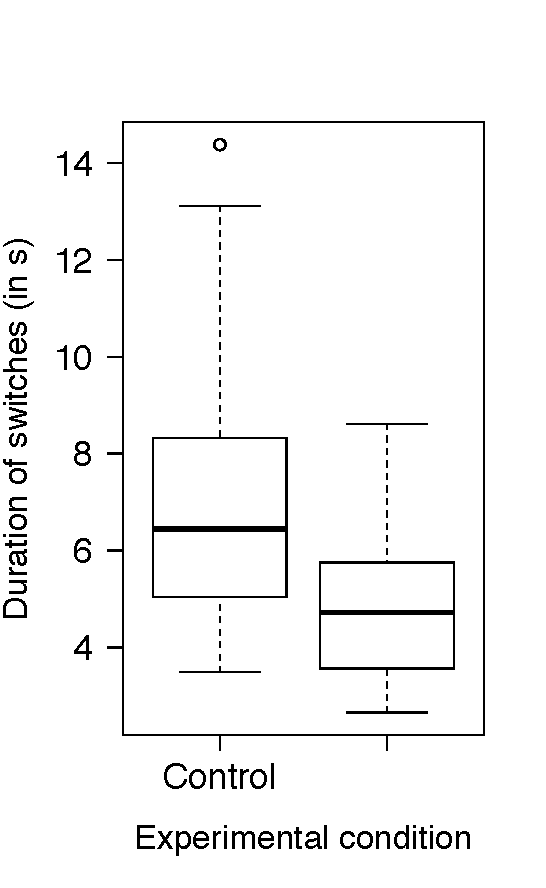
\includegraphics[width=0.2\textwidth]{images/ch56/ch56-boxplot.pdf}
\caption{Boxplot of duration of switches away from the data entry interface in each condition.}
%\vspace{-3pt}
\label{fig:ch56-Figure2}
\end{figure}

\subsubsection{Interkey intervals}
The primary measure to analyse switching behaviour were focus and blur events. These measures include any switch from the task window to another computer window, but task switches outside the device, with the task window still in focus, were not captured. Therefore, inter-keystroke interval (IKI) data was analysed to look for large intervals. The IKI data presented here does not make a distinction between moments when participants were inside or outside the task window, and longer intervals may have also been moments were participants had briefly paused for thought. However, extremely large intervals between two keystrokes might point to moments where participants had switched to doing something else. 

Figure \ref{fig:ch56-histikis} shows the distribution of IKIs. Table \ref{fig:ch56-tblswitches} shows the count of extremely long IKIs per condition.

\begin{figure}
\centering
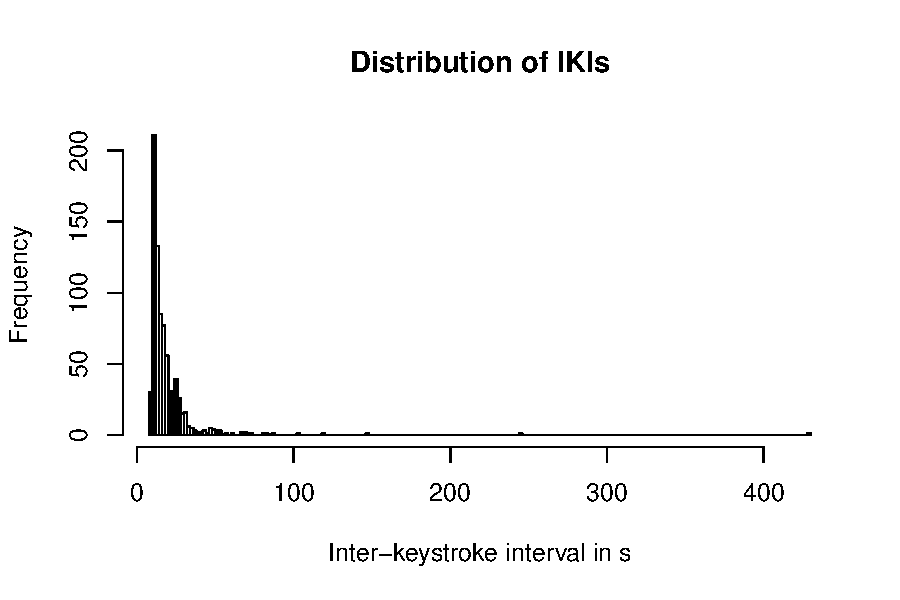
\includegraphics[width=\textwidth]{images/ch56/ch56-histikis.pdf}
\caption{Distribution of the top 10\% longest IKIs, that is IKIs that were longer than 6.21 seconds.}
%\vspace{-3pt}
\label{fig:ch56-histikis}
\end{figure}

\begin{table}
\caption{Total number of IKIs  at different percentiles for each condition.}
\centering
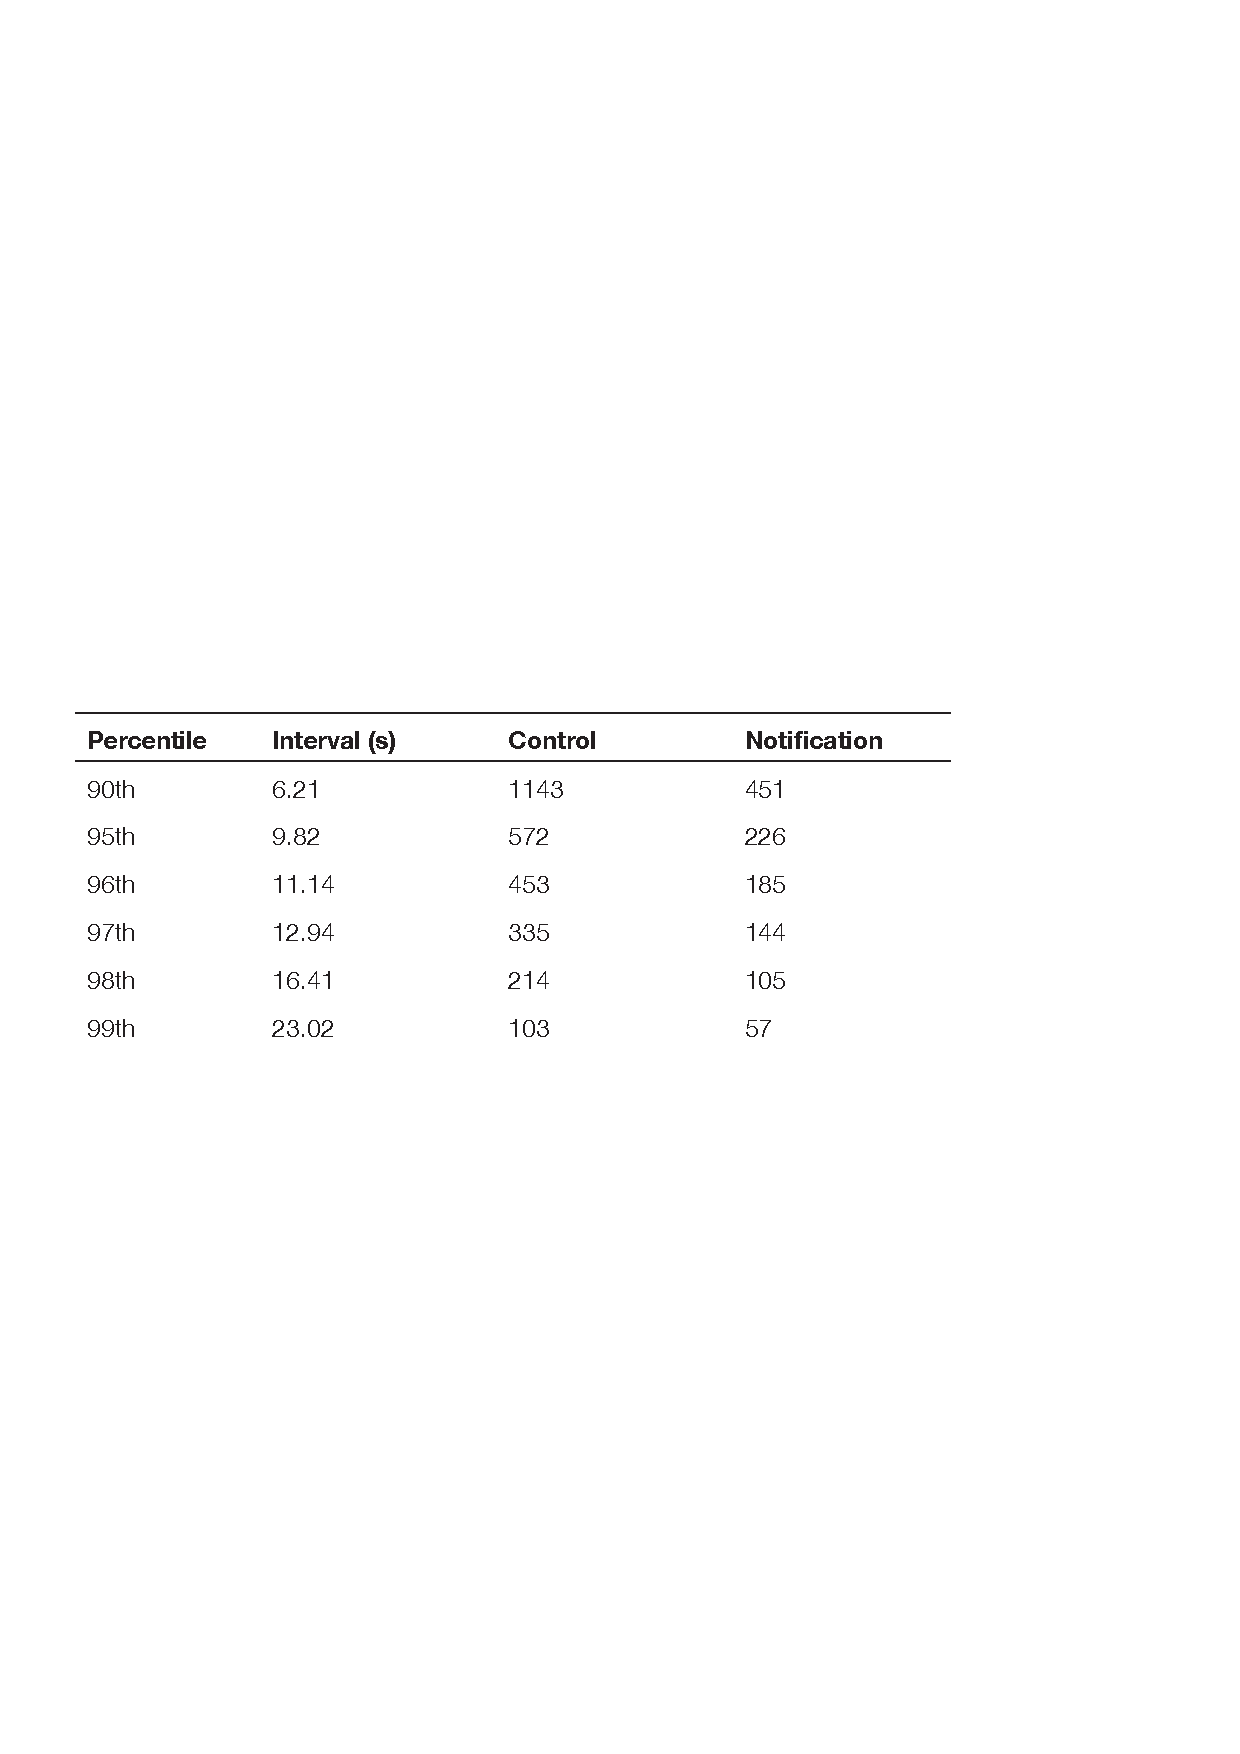
\includegraphics[width=0.7\textwidth]{images/ch56/ch56-longIKIs.pdf}
\vspace{-3pt}
\label{tbl:ch56-tblIKIs}
\end{table}

\subsection{Discussion}
The aim of this study was to see whether showing people how long they switch on average reduces the number and length of their switches. The results show that people can benefit from receiving feedback on the length of their switches: participants made shorter switches, were faster to complete the task, and made fewer errors. These findings suggest that shorter switches can lead to better task performance, and are in line with previous studies connecting the duration of an interruption to its disruptiveness \citep{Altmann2017, Monk2008}.

Nevertheless, as even short interruptions can have a negative effect on performance \citep{Altmann2014}, it was also measured if the number of switches were reduced. Interestingly, feedback on switching duration did not reduce the number of switches as in prior work \citep{Gould2016a}. This could be explained by the moment in the task that people received feedback. In Gould et al.'s study, feedback appeared after every switch. Participants may have tried to reduce switches, either because they were more aware of every switch or because they wanted to avoid the message. In contrast to our study, their participants were not supposed to switch, so the number of switches was lower. In the current study participants were switching more often as they had to as part of the task: on average, they switched once for every data entry (i.e., ten times per trial). Giving notifications at every switch would have had the risk of overexposing participants to notifications and limiting its usefulness \citep{Cutrell2001, Whittaker2016}. Therefore, feedback was only given after every trial. Future data entry studies that require fewer switches are needed to see if a notification upon every switch can reduce both the number and length of switches. Moreover, because the notification only showed information regarding the duration of switches, participants may have focused on reducing the duration, rather than number of switches. 

The current study used focus and blur events to analyse switching behaviour. This meant that task switches outside the device, with the task window still in focus, were not captured. Possibly participants learnt to not interrupt themselves when they were away from this window, but after they had returned to the window. Without an accurate estimate of how long participants should take to complete the task, it is difficult to determine moments at which participants were away from their computer \citep{Rzeszotarski2013}.  Using other techniques, such as prompts at random intervals to confirm people are still working on the task, may be able to give a further insight whether our intervention changes overall self-interruption behaviour. 

Most studies on self-interruptions introduced an artificial distraction, such as chat messages, to measure when, how long, and how often people self-interrupt to attend to this distracting task \citep{Katidioti2013, Salvucci2010}. The current study makes a methodological contribution by using participants' own personal email inbox, based on the assumption that email provides a source of distraction \citep{Hanrahan2015, Mark2016}. However, in the current study, participants only needed to find and open an email once. Once they had this email opened, they did not have to re-find it in their inbox for the remainder of the experiment, and may have had this email maximised on their screen, hiding incoming messages. In practice however, people have to first find the email in their inbox, which can partly contribute to the distraction. Our study has already shown an effect on behaviour by switching to an email inbox. It is expected there might be a higher potential for distraction if people have to also find the correct email in their inbox.

\subsubsection{Bridge to next study}
The results of this experiment indicate that showing people how long they switch on average reduces the duration of switches and can improve people's task performance. The work makes a contribution to our understanding of switching behaviour for routine data entry tasks to distracting, but task-relevant, applications such as email. The results also suggest ways in which tendencies to attend to distractions might be mitigated, and can provide a useful pointer for the design of productivity interventions to improve focus. In the current study, an experimental task was used in order to measure task performance. 

The study did not find any effect on the number of switches. However, as the number of switches indicate, participants presumably only switched to look up information, and did not switch to other tasks, interruptions or distractions. When people are doing their own data entry work, they may not have to switch as often as in the current experiment, but on the other hand they may interrupt themselves more to attend to other tasks and interruptions. To evaluate whether the positive effect of time feedback on people's switching behaviour can extend to naturalistic tasks, Study 7 tested the notification with office workers doing their own data entry work,

\section{Study 7: Looking up information for expenses in an office setting}

\subsection{Introduction}
%BRIDGE FROM LAST STUDY
%Study 6 aims to evaluate the design recommendations in a finance office with workers, to see how appropriate and feasible the proposed recommendations would be in the context for which they are developed. Depending on what the design recommendations will be, I will take them through a prototype, which can be a paper prototype, storyboard, or digital mockup, and if possible I will ask them to perform the task with and without the proposed changes. 

In order to understand whether the notification would have the same effect on a naturalistic data entry task, Study 6 was followed up with a field study testing the notification with data entry workers doing expenses work. To measure self-interruption behaviour during their work, participants were asked to install a free trial version of ManicTime \footnote{https://www.manictime.com} for two weeks. ManicTime is a time tracking software, which tracks application and web page usage. In addition, half of the participants were asked to install a browser extension, and use it when they are processing expenses. Every time participants switched away from the browser window in which they did their expenses work, the extension showed a notification similar to the notification used in Study 6. The purpose of the study was to see whether a notification had an effect on self-interruption behaviour. To get a quantitative measure of self-interruption behaviour, ManicTime data was used to derive number and duration of window switches during expenses work. In addition, participants were interviewed to explore whether and how the use of both the extension and ManicTime led to any conscious changes in their behaviour.
 
The study aims to address the following research question: how does feedback on interruption length have an effect on people's self-interruption behaviour during expenses work in a finance office setting? 

\subsection{Focus, a browser extension}
%Include implementation details
The browser notification was implemented as a Google Chrome extension, using HTML, Javascript and CSS. Participants were sent a link to download the extension, named Focus, and were given instructions to install and add it to their Google Chrome browser. To use the extension, participants had to navigate to the web page in their Google Chrome browser where they had to complete their work and click on the icon of the extension. As was found in Study 1 and 2, the majority of data entry work studied in this thesis, such as processing expenses, was done in a web browser. Upon clicking on the icon, a pop-up appeared saying that the current web page was now the main task page. Every time participants switched away from this page, they received a notification indicating how long their switches away from this page are on average. Participants could stop the notifications by refreshing or closing the page. 

The main difference in notification behaviour with respect to Study 6 was that participants received the notification every time they switched away from their task window, rather than at particular moments in the task. They only received it when they switched away from their task window, but not upon any subsequent switches. Furthermore, due to security issues the extension did not store any data. Instead, the application ManicTime was used to measure people's switching behaviour. 


\subsection{Method}
%DESIGN
To study the effect of a notification on people's self-interruption behaviour, a between-groups design was used and participants were divided into a control group and experimental group. The control group was asked to install ManicTime for two weeks. They were told the purpose of the study was to understand how people in offices manage tasks, windows and applications. The experimental group additionally were asked in the second week to install Focus. They were told that this extension would give additional information on the current task they were working on. Other than this distinction, all instructions were identical between the two groups. 

Four participants were unable to use Google Chrome, and therefore the extension, for their work. Therefore, these participants were part of the control group. To make the groups even, one other participant was randomly chosen to be allocated to the control group; the remaining participants were allocated to the experimental group. 

%If the main task page is not in focus, either because participants have switched to another page or if it has been inactive for x seconds, they will receive a notification with a warning message. Upon returning to the expenses page, they will receive a notification indicating how long they were away from the page. The control group will be asked to install the plug-in, but will receive no notifications. It is explained that the purpose of the study is to log people's switching behaviour, and participants will be able to see their data at the end of the study. Participants will be asked to use the add-in for one week in which they have to do a substantial amount of expenses work, and keep a diary of their experiences. Within a week of finishing the diary, a follow-up interview will be scheduled to gather more detailed explanations of participants' experiences of using the add-in.

\subsubsection{Participants}
Ten participants (three male) took part in the study. They were recruited using the same recruitment methods as Study 1 and 2. Invitations were sent to opt-in mailing lists of Finance departments of a university, and forwarded by contact persons and people who had already participated. None of the participants had taken part before in any of the studies reported in this thesis, but were drawn from the same population. None of the participants had used a time management application such as ManicTime before. Participants were reimbursed with a \pounds 20 Amazon voucher.

\subsubsection{Procedure}
Participants who expressed interest were sent an information sheet and consent form to read and sign. They were sent an overview of the study, instructions to install the tools, and a post-study interview was scheduled.
The study was divided into three stages:
\paragraph{Week 1: Install ManicTime}
In the first week, participants were sent instructions to install ManicTime on their work computer. They were given the option to pause or stop the application from running at any time. They were told that they were free to choose if, when and how often to look at the information, but that it was important to complete at least one expenses task with the application running. 

\paragraph{Week 2: Install Focus}
In the second week, participants in the experimental condition were asked to install Focus. Again, they were instructed that they were free to choose when and how often to use the extension, but that they had to use it for at least one expenses task. Even though the second week was the same for participants in the control condition, they were also asked to complete at least one expenses task in the first week, and another expenses task in the second week. This instruction was included to compare if any observed changes in switching behaviour were due to the browser extension, or if participants simply became more aware of their switching behaviour in the second week.

\paragraph{Week 3: Interview}
%Participants were sent an email with instructions on how to share their database and remove the tools from their computer.
In the third week, participants were interviewed about how they currently manage documents, applications and tasks for their work, and asked questions on their experience of using the tools. In particular, it was discussed whether and how they used or would use the information that the tools provided, and whether they made any changes on how they went about their work. They were asked to share their ManicTime database for further analysis. Participants were offered guidance and assistance on deleting or adapting any data in their database, such as removing application and website names. Participants were still eligible to participate, if they did not wish to share their database.

The interviews took place in a closed room , lasted about 50 minutes and were audio recorded.

\subsubsection{Pilot study}
A pilot study was conducted with two participants. One participant was a colleague and was sent instructions to install Focus on his computer. The purpose of this pilot session was to see whether the installation instructions were clear and to test the extension on other people's computers. The participant had the tendency to hover over the notification to stop it from disappearing, which placed extra buttons over the end of the notification message. Therefore, the message was shortened and the most important information, namely the duration of switches, was placed at the front of the message to ensure it was still visible upon hovering.

A second pilot session was then conducted with an administrator working at the same university as the study participants, who was asked to install ManicTime and Focus on her work computer. The purpose of this session was to ensure the tools could be installed on the work computers of the university, and that the extension worked with the university finance system.

%Findings pilot study

\subsubsection{Ethical considerations}
Participants were informed before undertaking the study that they would be asked to share their ManicTime database at the end of the study. However, a disclaimer was added in the invitation and instruction emails that participants were still able to take part, if they did not wish to share their database. It was made clear what data ManicTime recorded, and that Focus did not store any data. They were given instructions on how to pause the application from running and how to delete certain parts of the data, and were offered assistance to help further change the database into a state they were comfortable sharing. 

\subsubsection{Data analysis}
Though ManicTime was piloted on a work computer of the university before starting the study, three participants were unable to install ManicTime on their work computer due to firewall restrictions. Furthermore, two participants opted out of using Focus as they used a browser different from Google Chrome for at least parts of their work. Therefore, ManicTime data of the remaining four participants was used to complement qualitative explanations of their task switching behaviour, but it was not analysed quantitatively as previously planned to compare switching behaviour with and without the extension. Instead, the primary focus of data analysis was on the post-study interviews and participants' subjective experience of using the tools. The interviews were trancsribed verbatim, and analysed using thematic analysis.

%Four participants successfully installed and used ManicTime, and two participants used Focus. 

\subsection{Findings}
%Reflective and current information
\subsubsection{Reflective information}
Participants made to-do lists and schedules, but did not look back at them. P2 did look back at them, but only to move forward tasks he had not finished, and not to adjust expectations on his time management. They found it more useful to get information on current behaviour, as they did not know what to do with reflective information. 

P3 would like to look back, and tried to with ManicTime, but felt it was effortful and did not have the time to reflect on it:

\textit{'I don't have time that I can set aside to work on things that will help me later (…). the only period where I would have the time to do these things, is when I get home. And when I get home, I'm at home, and I just can't be bothered doing more work stuff.'} (P3)

%Prospective information; Use of to-do lists, schedules
\subsubsection{Prospective information: to-do lists and schedules}
Participants used prospective time information: they made written to-do lists but did not allocate time or deadlines to these. To-do lists were used to write down specific tasks without a time allocation. Schedules were used to allocate time blocks to higher-level tasks. P2 set aside several hours to work on `finance-related' tasks, or email.

%Digital vs. non-digital interruptions
\subsubsection{Type of interruptions}
\paragraph{Digital versus non-digital interruptions}

Participants discussed that the information Focus provided would be useful, but that it currently did not capture the full data as it only looked at digital interruptions. Upon the first time of switching windows, the notification would say there was no interruption data yet: 

\textit{`That's when I sort of thought: `Oh, that's not really saying much, is it? Because it's not actually true. Because of course there were interruptions.''} (P2)

P1 and P2 said that they had just as much digital as non-digital interruptions, that these were equally disruptive, and felt that time data on digital switches only told part of the story. It would be useful to get information on both of these interruptions.

All participants found the timeline that ManicTime provided on time active and away from the computer useful.

P2 would use it to schedule in more breaks, whereas it made P3 realise his breaks were much longer than he thought:

\textit{`when I'm going to print something, and I end up talking with someone, and I come back, and it's like: you've been out for half an hour. And I was like: Jesus, time's flying! No wonder I work until 6 every day.'} (P3)

Participants did not find a list of applications useful, as they spent the most time in the same applications. P2 and P3 only looked at it out of curiousity, but did not see the use of it for work. 

\subsubsection{Physical environment}
Participants did not always work in the same location. For example, P3 worked in two different offices, and all participants worked from home occasionally. Different environments introduced different types of interruptions. 

%Working from home; gaps in reflective data
\subsubsection{Gaps in data}
X participants worked days from home, which left gaps in the ManicTime data.


\subsubsection{Time feedback}
Participants were particularly interested in the time it took them when they were not at their task. For P3, it helped him take shorter and fewer breaks:

\textit{`it made me realise how long I was spending, spending/wasting, doing other stuff. I think that affected me in the sense that I wanted to take fewer breaks. Because I didn't, well by breaks I mean, as I told you earlier, it's just going to do something, and then ending up chatting with someone in the passing.'} (P3)

However, for other people it was not surprising:

\textit{`I don't really know whether that's helpful. To me, it doesn't kind of make me think: 'Oeh, I've been away too long'. I just think: OK, well I'm roughly aware that I've been away for an hour (…), I don't see how it links with being more productive. Unless I suppose, you're really easily distracted.'} (P7) 

\subsubsection{Switching between windows}
Participants did not find it useful to see how much time they spend in certain applications or windows. P2 was curious, but did not find it surprising as he spends most time in the information systems he uses for work, which are the main task windows. 
Most tasks revolved around a main task window, and participants found it easy to select one. 
%Whittaker and Collins found that people think in time on tasks, not time on specific document. We found people think more in 'time on work, or specific type of work'. They do think in tasks but do not put time on it. 

\subsubsection{Distractions}

\subsection{Discussion}

\subsection{Limitations}
%Unable to use ManicTime data

\subsection{Contributions}
\begin{itemize}
\item
Development of design recommendations for an expenses system.
\item
Demonstrate how an understanding of the used information sources and people's switching strategies between entering and looking up information can be used to adapt the design of the data entry interface. 
\item
Demonstrate the applicability of design recommendations in the financial office settings in which the expenses task is currently done. 
\item
Demonstrate that design features can influence people's strategies in entering expenses in a financial office setting.
\end{itemize}

